\documentclass[tikz,border=7pt]{standalone}
\usetikzlibrary{arrows.meta,calc}

% Edit these four scalars to change each plane's dilation state.
% Each plane's in-plane coordinate extent is multiplied by its gamma value.
\def\gammaA{1.00}
\def\gammaB{1.15}
\def\gammaC{1.30}
\def\gammaD{1.45}

\tikzset{
  plane grid/.style={line width=0.35pt},
  plane outline/.style={line width=0.8pt},
  axis/.style={-{Stealth[length=2.2mm,width=1.7mm]},line width=1.1pt},
  plane label/.style={
    font=\small,
    fill=white,
    fill opacity=0.92,
    text opacity=1,
    inner sep=2pt
  },
}

% #1 plane index, #2 stack coordinate, #3 dilation scalar, #4 color
\newcommand{\DrawPlane}[4]{%
  \pgfmathsetmacro{\g}{#3}%
  % The plane is a square in its own (x^1,x^2) coordinates.
  \path[fill=#4!11,draw=#4!75!black,plane outline]
    (-\g,-\g,#2) -- (\g,-\g,#2) -- (\g,\g,#2) -- (-\g,\g,#2) -- cycle;

  % Same normalized grid on every plane.
  \foreach \f in {-1,-0.5,0,0.5,1}{%
    \pgfmathsetmacro{\u}{\f*\g}%
    \draw[#4!58!black,plane grid]
      (\u,-\g,#2) -- (\u,\g,#2);
    \draw[#4!58!black,plane grid]
      (-\g,\u,#2) -- (\g,\u,#2);
  }%

  \fill[#4!80!black] (0,0,#2) circle[radius=1.1pt];

  \node[plane label,anchor=west] at (2.15,-1.55,#2)
  {$l_{#1}=\pgfmathprintnumber[fixed,precision=2]{\g}$};
}

\begin{document}

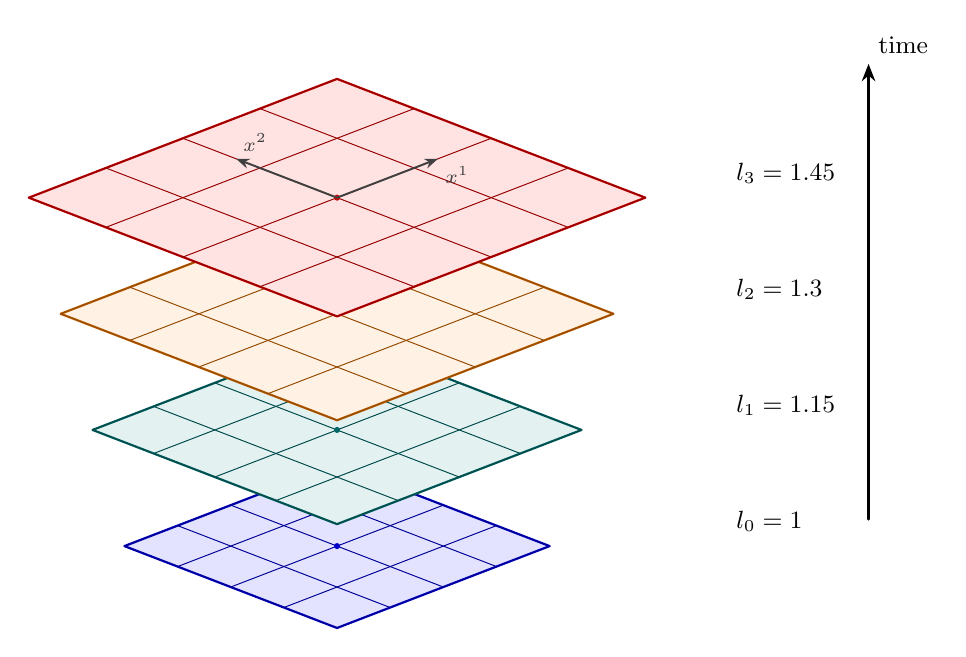
\begin{tikzpicture}[
  x={(1.35cm,0.52cm)},
  y={(-1.35cm,0.52cm)},
  z={(0cm,1.18cm)},
  line join=round,
  line cap=round,
  font=\sffamily,
]

  % Orthogonal basis in the represented geometry.
  % x^1 and x^2 span a plane; z is its perpendicular stack direction.
  % The drawing uses an oblique projection.

  \DrawPlane{0}{0.00}{\gammaA}{blue}
  \DrawPlane{1}{1.25}{\gammaB}{teal}
  \DrawPlane{2}{2.50}{\gammaC}{orange}
  \DrawPlane{3}{3.75}{\gammaD}{red}

  % Time is shown as an ordering parameter along the perpendicular stack axis.
  \draw[axis,black]
    (3.0,-2.0,-0.15) -- (3.0,-2.0,4.75);

  \node[anchor=west,align=left,font=\small]
    at (3.0,-2.0,4.95)
    {time};

  % Coordinate-direction indicators on the upper plane.
  \draw[-{Stealth[length=1.7mm]},line width=0.7pt,black!75]
    (0,0,3.75) -- (0.95,0,3.75)
    node[below right=-1pt,font=\scriptsize] {$x^1$};

  \draw[-{Stealth[length=1.7mm]},line width=0.7pt,black!75]
    (0,0,3.75) -- (0,0.95,3.75)
    node[above right=-1pt,font=\scriptsize] {$x^2$};

\end{tikzpicture}

\end{document}
